\section{Increasing the Instruction Set (Augmentation du Jeu d'Instruction)}
\label{sec:Increasing the Instruction Set (Augmentation du Jeu d'Instruction)}

In this section, we have added additional command suffix support, including \texttt{EQ, NE, LT, GT}.
The detailed information is given in Table \ref{tab:Condition Code}.

\begin{table}[htbp]
    \centering
    \caption{Condtion Code}
    \label{tab:Condition Code}
    \begin{tabular}{@{}cccc@{}}
    \toprule
    \textbf{Code} & \textbf{Suffix} & \textbf{Flag} & \textbf{Meaning} \\ \midrule
    0000          & EQ              & Z=1           & equal            \\
    0001          & NE              & Z=0           & not equal        \\
    1011          & LT              & N=1           & less than        \\
    1100          & GT              & N=0           & greater than     \\ \bottomrule
    \end{tabular}
\end{table}

In order to match these changes, we need to modify the codes we have done before such as \textbf{ALU.vhd}, \textbf{Decoder.vhd} and \textbf{Data\_memory.vhd}
and rewrite the instructions in \textbf{instruction\_memory3.vhd}.

For \textbf{ALU.vhd}, we add an additional output port \texttt{Z} which indicated ZERO in Status.

For \textbf{Decoder.vhd}, we add the branch of \texttt{case} to make it decoder \texttt{EQ, NE, LT, GT} successfully
according to Table \ref{tab:Condition Code}.

For \textbf{Data\_memory.vhd}, we add the initialization for datas in memory as Table \ref{tab:datas in mem}.
\begin{table}[htbp]
    \centering
    \caption{Datas in Memory}
    \label{tab:datas in mem}
    \begin{tabular}{@{}cc@{}}
    \toprule
    \textbf{Address} & \textbf{Data} \\ \midrule
    0x20          & 3              \\
    0x21          & 107              \\
    0x22          & 27              \\
    0x23          & 12              \\
    0x24          & 322              \\
    0x25          & 155              \\
    0x27          & 63              \\ \bottomrule
    \end{tabular}
\end{table}

Finally, we created the command in \textbf{instruction\_memory3.vhd} as below.
\begin{lstlisting}[style=vhdl, columns=fixed]
result (0) :=x"E3A00020";-- 0x0 _start    -- MOV R0,#0x20
result (1) :=x"E3A02001";-- 0x1	          -- MOV R2,#1
result (2) :=x"E3A02000";-- 0x2 _while    -- MOV R2,#0
result (3) :=x"E3A01001";-- 0x3		      -- MOV R1,#1
result (4) :=x"E6103000";-- 0x4 _for      -- LDR R3,[R0]
result (5) :=x"E6104001";-- 0x5	    	  -- LDR R4,R0,#1
result (6) :=x"E1530004";-- 0x6		      -- CMP R3, R4
result (7) :=x"C6004000";-- 0x7	    	  -- STRGT R4,[R0]
result (8) :=x"C6003001";-- 0x8	    	  -- STRGT R3,[R0,#1]
result (9) :=x"C2822001";-- 0x9		      -- ADDGT R2,R2,#1
result (10):=x"E2800001";-- 0xA           -- ADD R0, R0, #1
result (11):=x"E2811001";-- 0xB           -- ADD R1, R1, #1
result (12):=x"E3510007";-- 0xC           -- CMP R1, #0x07
result (13):=x"BAFFFFF6";-- 0xD           -- BLT FOR
result (14):=x"E3520000";-- 0xE           -- CMP R2, #0
result (15):=x"E3A00020";-- 0xF           -- MOV R0, #0x20
result (16):=x"1AFFFFF1";-- 0x10          -- BNE WHILE        
result (17):=x"EAFFFFFF";-- 0x11 _wait    -- BAL wait	     
\end{lstlisting}

After running the testbench with command file \textbf{Processor\_test.do}, we obtain the waves as Figure \ref{fig:PUEXres}.
\begin{figure}[htp]
    \centering
    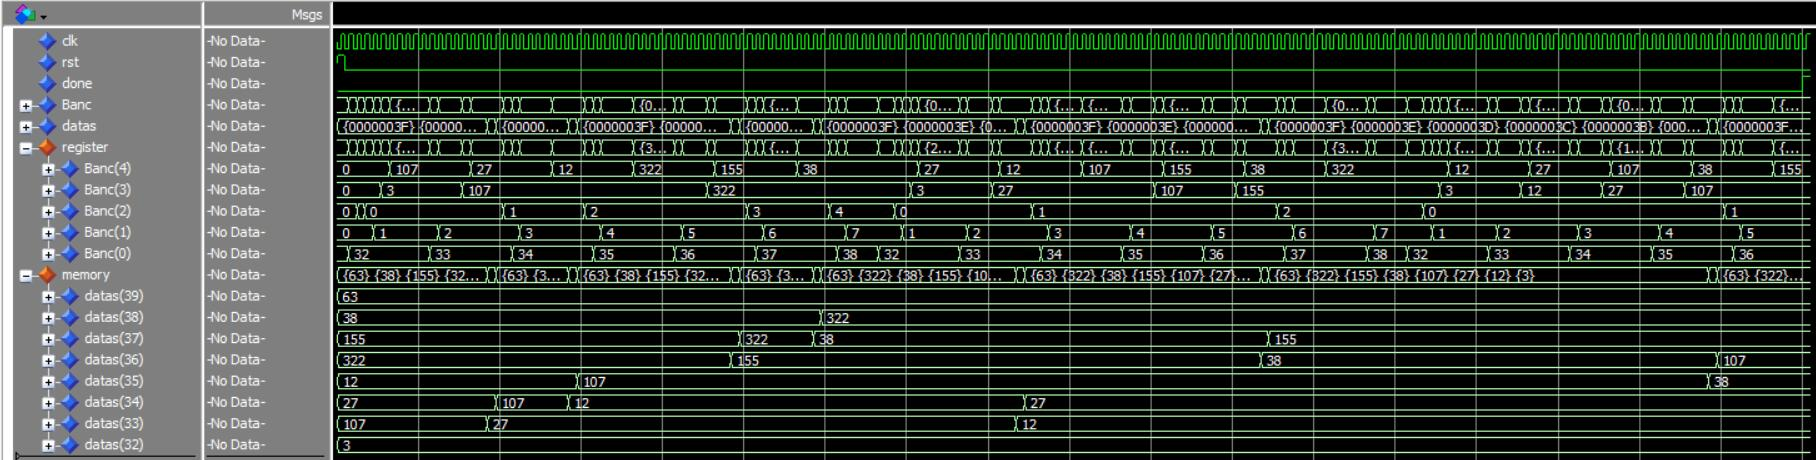
\includegraphics[width=1\textwidth]{picture/PUEXres.jpg}
    \caption{Simulation Waves of Processing Unit with IS Increasing}     
    \label{fig:PUEXres}
\end{figure}








